% main.tex -- paper/v1: faithful LaTeX reconstruction of the draft PDF
% context/esann2027_paper_draft.pdf (6 pages, pdfTeX 1.40.25, 2026-10-15),
% whose source is lost.  Phase L1, 2026-11-09.  Wording, numbers, notation,
% floats and references reproduce the draft; do not edit this file for the
% revision (it is the baseline to diff against).
%
% Build:  cd paper/v1 && latexmk -pdf     (self-contained folder: esannV2.cls
%         here is a byte-identical copy of the official ../esannV2.cls, and
%         fig1_interaction.pdf a copy of ../../analysis/fig1_interaction.pdf as
%         used in the draft)
% Check:  main.pdf matches the draft glyph for glyph (0.000 bp) on all 6 pages;
%         only the itemize bullets differ (Type 1 vs the draft's Type 3 bitmap).
% Notes:  reports/latex_notes.md
\documentclass{esannV2}
% The template loads graphicx with [dvips]; under pdflatex that option drops
% every figure ("Non-PDF special ignored!"), so it is loaded without option.
\usepackage{graphicx}
% The template's \usepackage[latin1]{inputenc} is omitted: this source is pure
% ASCII and LaTeX >= 2018 reads UTF-8 by default.
\usepackage{amssymb,amsmath,array}
\usepackage{booktabs}
\usepackage{url}

% esannV2.cls never sets the PDF page size (its default option "a4" is not a
% declared option), so the size would come from the local TeX configuration.
% ESANN requires A4: fix it explicitly (same size as the draft).
\ifdefined\pdfpagewidth \pdfpagewidth=210mm \pdfpageheight=297mm \fi

%***********************************************************************
% Template block, unchanged: margins are those of esannV2.cls.
\voffset 0 cm \hoffset 0 cm \addtolength{\textwidth}{0cm}
\addtolength{\textheight}{0cm}\addtolength{\leftmargin}{0cm}
%***********************************************************************

\begin{document}

\title{Do Pruning and Quantization Compose? Order and Interaction in
Post-Training Compression of Language Models}

%***********************************************************************
% AUTHORS INFORMATION AREA
%***********************************************************************
\author{[Authors and affiliations to be confirmed]}
%***********************************************************************
% END OF AUTHORS INFORMATION AREA
%***********************************************************************

\maketitle

\begin{abstract}
Post-training pruning and quantization are routinely stacked to compress
language models, under the implicit assumption that their errors are
independent. We test this assumption inside one optimal-brain-surgeon
framework, comparing joint, prune-then-quantize and quantize-then-prune
compression at equal storage cost on three models (135M--0.5B), and we
re-analyse published 7--8B results. A decomposition of the layer error
predicts sub-additivity whenever the pruning mask is chosen before the
quantization grid. Experiments confirm it in all 36 mask-first cases.
Quantizing first is super-additive at 4 bits and gives the worst perplexity
in 16 of 18 settings, up to twice the best one.
\end{abstract}

\section{Introduction}

Pruning removes weights; quantization shortens the remaining ones. Both have
accurate one-shot, post-training versions for large language models (LLMs)
built on the same second-order principle: SparseGPT~\cite{frantar2023sparsegpt}
for pruning and GPTQ~\cite{frantar2023gptq} for quantization, both descendants
of Optimal Brain Surgeon (OBS)~\cite{lecun1990obd,hassibi1993obs}. Stacking
them is attractive because the gains multiply~\cite{han2016deep}. In earlier
work~\cite{laborde2025semantic} we showed that, at an equal theoretical
compression rate (TCr), 25\% pruning with 4-bit quantization retains about
20\% more performance than pure 3-bit quantization on 7--8B models. That
study, like most practice, applied the two methods one after the other and
assumed that their errors do not interact.

This assumption is not innocuous. Harma et al.~\cite{harma2025effective}
proved that sparsity and max-scaled quantization are non-orthogonal and that
sparsity should come first. Joint methods~\cite{guo2024jsq,guo2025obr} report
that naive stacking leaves accuracy on the table. What is missing is a direct
measurement, inside the Hessian-based post-training pipeline used in practice,
of \emph{how} the two errors combine and of whether the answer depends on
model size.

We answer three questions. \textbf{Q1:} is the combined layer error the sum
of the individual errors? \textbf{Q2:} at fixed TCr, does the order of the
operations matter? \textbf{Q3:} does the interaction change with scale? Our
contributions are: (i) a single OBS sweep that implements pruning,
quantization and their three combinations with identical machinery, so that
only the order differs; (ii) a decomposition of the combined layer error that
explains when it is sub-additive; (iii) a controlled study of 93 runs on three
models (135M--0.5B) on a free GPU, complemented by a re-analysis of the
published 7--8B results of~\cite{laborde2025semantic}.

\section{One framework for pruning, quantization and their combinations}
\label{sec:framework}

For a linear layer with weights
$W\in\mathbb{R}^{d_{\mathrm{out}}\times d_{\mathrm{in}}}$ and calibration
inputs $X$, post-training compression solves
$\min_{\widehat W}\|WX-\widehat W X\|_F^2$ under a sparsity or precision
constraint. With $H=2XX^\top$ and $\Delta=W-\widehat W$, the objective is
$\mathrm{tr}(\Delta H\Delta^\top)$, and we report the normalized layer
error $E(\widehat W)=\mathrm{tr}(\Delta H\Delta^\top)/\mathrm{tr}(WHW^\top)$.
OBS-type methods process the input columns in order. When column $j$ is
replaced by its compressed value, the error is propagated to the remaining
columns through the inverse Hessian, so later columns compensate for earlier
decisions. SparseGPT zeroes, per block of 128 columns, the weights with the
smallest saliency $w^2/[H^{-1}]_{jj}^2$; GPTQ rounds each column to a min--max
asymmetric grid fitted per row and per group of 128 columns. We implement both
as options of one sweep and define three combinations:

\begin{itemize}
\item \textbf{Joint} (as in~\cite{frantar2022obc,frantar2023sparsegpt}): one
  sweep; in each block the mask is selected first, the grid is fitted on the
  kept weights, then every column is pruned and quantized before
  compensation.
\item \textbf{P$\to$Q}: a pruning sweep returns $W_P$ and its mask $M$; a
  quantization sweep on $W_P$ keeps $M$ fixed, so pruned weights stay exactly
  zero while their error is still compensated.
\item \textbf{Q$\to$P}: a quantization sweep returns $W_Q$ and its grid $G$; a
  pruning sweep on $W_Q$ selects the mask and projects every compensated
  weight back onto $G$.
\end{itemize}
All three have the same storage cost. With sparsity $s$ and bit-width $b$
(16-bit baseline), $\mathrm{TCr}=1-\frac{b}{16}(1-s)$~\cite{laborde2025semantic}.
Joint and P$\to$Q are \emph{mask-first}: the mask is known when the grid is
fitted. Q$\to$P is \emph{grid-first}. Layers are compressed sequentially, each
calibrated on the outputs of the already-compressed previous layers.

\section{Measuring interaction}
\label{sec:interaction}

\textbf{Layer level.} Let $E_P$, $E_Q$ and $E_{PQ}$ be the layer errors of
pruning only, quantization only and a combination. The combination is
\emph{additive} if $E_{PQ}=E_P+E_Q$; we define the interaction
$I_E=E_{PQ}-(E_P+E_Q)$.

\textbf{Decomposition.} Write $\langle A,B\rangle_H=\mathrm{tr}(AHB^\top)$
and $\|A\|_H^2=\langle A,A\rangle_H$. Consider a mask $M$ and a fixed grid
$q(\cdot)$ without compensation. Let $P=W\odot M$ be the pruned weights and
$R=W-q(W)$ the rounding residual, split as $R=R_M+R_{\bar M}$ on the pruned
and kept entries. Then $\Delta_P=P$, $\Delta_Q=R$ and $\Delta_{PQ}=P+R_{\bar M}$,
which gives, up to the common normalization,
\[
  I_E \;\propto\; \underbrace{-\,\|R_M\|_H^2}_{\text{absorption}\;\le\;0}
  \;+\; \underbrace{2\langle P,R_{\bar M}\rangle_H
  -2\langle R_M,R_{\bar M}\rangle_H}_{\text{cross terms}}.
\]
The first term is never positive: rounding errors on weights that are pruned
anyway disappear. Because $P$, $R_M$ and $R_{\bar M}$ have disjoint supports
within each row, both cross terms vanish when $H$ is diagonal, i.e.\ when
input features are uncorrelated. In that case $E_{PQ}\le E_P+E_Q$:
\emph{pruning and quantization are sub-additive}. The absorption argument
requires that the grid can represent the pruned state; a mask-first order
fits the grid to the kept weights, whereas a grid-first order forces the
compensated kept weights back onto a grid fitted before pruning, which adds
rounding error outside this decomposition. We therefore expect mask-first
orders to be sub-additive and the grid-first order to lose this guarantee.
With OBS compensation the residuals no longer have these closed forms, so
Section~\ref{sec:results} tests the prediction.

\textbf{Model level.} With semantic retention $Sr$, the ratio of compressed to
original performance summed over tasks~\cite{laborde2025semantic},
independent degradations multiply. We use $I_{Sr}=Sr_{PQ}-Sr_P\,Sr_Q$; a
positive value means the combination does better than independence predicts.

\section{Experimental setup}
\label{sec:setup}

We compress SmolLM2-135M and -360M~\cite{benallal2025smollm2} and
Qwen2.5-0.5B~\cite{qwen2024qwen25}: all linear layers of all decoder blocks;
embeddings and output head stay in 16 bits. Calibration uses 128 random
windows of 2048 tokens from C4~\cite{raffel2020t5}, damping
$0.01\,\overline{\operatorname{diag}(H)}$, blocks and groups of 128 columns.
The grid crosses $s\in\{25,33.3,50\}\%$ with $b\in\{4,3\}$, each in the three
orders, plus single-method baselines ($b=8$ included): 25 models per network.
We report WikiText-2~\cite{merity2017pointer} perplexity (2048-token windows)
and zero-shot accuracy on ARC-Easy~\cite{clark2018arc}, PIQA~\cite{bisk2020piqa}
and HellaSwag~\cite{zellers2019hellaswag} (first 500 items each) with
lm-eval~\cite{gao2024lmeval}. On SmolLM2-135M, 18 extra runs repeat the key
cells with two more calibration seeds. Everything runs on free T4 GPUs in
16-bit; six SmolLM2-360M runs that overflowed were repeated in 32-bit (three
16-bit controls repeated in 32-bit differ by at most 0.4\% in perplexity).
Unit checks run at every layer: exact mask ratio, pruned weights still zero
after quantization, at most $2^b$ levels per group, and exact reproduction of
the dense forward pass. Code and raw results:
\url{https://github.com/antounyaacoub/esann2027-compose}
(DOI 10.5281/zenodo.23396063).

\begin{figure}[t]
\centering
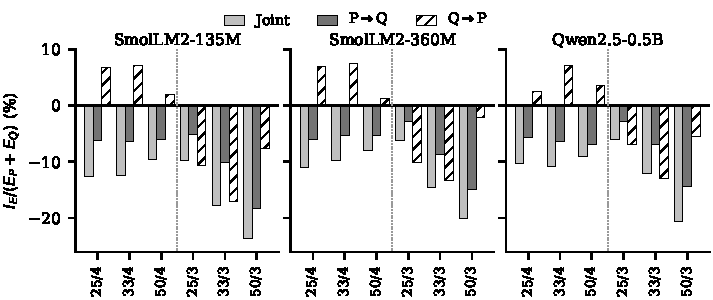
\includegraphics[width=\textwidth]{fig1_interaction}
\caption{Layer-level interaction $I_E$, relative to the additive prediction
$E_P+E_Q$ (mean over all linear layers), for each model and each cell
($s$/$b$). Negative: sub-additive.}
\label{fig:interaction}
\end{figure}

\section{Results}
\label{sec:results}

\textbf{Q1: mask-first orders are sub-additive.} Fig.~\ref{fig:interaction}
shows the relative interaction in all 54 combined models. Both mask-first
orders are sub-additive in every one of the 36 cases: by 6--24\% for the
joint sweep and 3--18\% for P$\to$Q. The grid-first order Q$\to$P is
super-additive in all nine 4-bit cases (+1 to +7\%), as the decomposition
predicts once the grid no longer matches the kept weights. At 3 bits Q$\to$P
becomes sub-additive for a different reason: 3-bit rounding already sets
31--33\% of the weights exactly to zero (15--17\% at 4 bits), so a grid-first
pruning of 25\% only selects weights that are already zero. The resulting
model is identical to 3-bit quantization alone ($E_{PQ}=E_Q$, $I_E=-E_P$, same
perplexity on all three networks): absorption in its extreme form. The TCr
formula, which counts the two compressions independently, misses this free
sparsity.

\begin{table}[t]
\centering
{\footnotesize
\setlength{\tabcolsep}{3.5pt}
\begin{tabular}{llc|cc|ccc}
\toprule
Model & $s$ + $b$ & TCr & $P$ only & $Q$ only & Joint & P$\to$Q & Q$\to$P \\
\midrule
% Body rows: copied verbatim from analysis/table1_rows.tex (written by
% analysis/reproduce_paper.py) and checked against the draft PDF, 2026-11-09.
SmolLM2-135M & 25\% + 4 & 0.812 & 16.48 & 21.77 & 23.04 & \textbf{21.86} & 24.03 \\
(dense 15.42) & 33\% + 4 & 0.833 & 18.39 & 21.77 & 26.08 & \textbf{24.11} & 27.73 \\
 & 50\% + 4 & 0.875 & 32.89 & 21.77 & 45.45 & \textbf{40.15} & 49.68 \\
 & 25\% + 3 & 0.859 & 16.48 & 58.17 & 60.87 & \textbf{56.88} & 58.17 \\
 & 33\% + 3 & 0.875 & 18.39 & 58.17 & 63.18 & \textbf{58.97} & 68.00 \\
 & 50\% + 3 & 0.906 & 32.89 & 58.17 & \textbf{88.24} & 97.97 & 150.10 \\
\midrule
SmolLM2-360M & 25\% + 4 & 0.812 & 12.07 & 13.29 & \textbf{13.17} & 13.32 & 14.34 \\
(dense 11.46) & 33\% + 4 & 0.833 & 12.86 & 13.29 & \textbf{14.12} & 14.20$^{*}$ & 15.53 \\
 & 50\% + 4 & 0.875 & 18.64 & 13.29 & \textbf{20.82} & 21.02 & 23.82 \\
 & 25\% + 3 & 0.859 & 12.07 & 25.92 & \textbf{20.11}$^{*}$ & 20.77 & 25.92 \\
 & 33\% + 3 & 0.875 & 12.86 & 25.92 & \textbf{20.34}$^{*}$ & 20.88 & 30.50$^{*}$ \\
 & 50\% + 3 & 0.906 & 18.64 & 25.92 & \textbf{28.71}$^{*}$ & 30.07$^{*}$ & 57.80 \\
\midrule
Qwen2.5-0.5B & 25\% + 4 & 0.812 & 13.63 & 14.24 & \textbf{14.68} & 14.71 & 15.02 \\
(dense 13.07) & 33\% + 4 & 0.833 & 14.52 & 14.24 & \textbf{15.62} & 15.69 & 15.99 \\
 & 50\% + 4 & 0.875 & 20.21 & 14.24 & \textbf{21.61} & 22.44 & 22.74 \\
 & 25\% + 3 & 0.859 & 13.63 & 21.95 & 21.96 & 22.11 & \textbf{21.95} \\
 & 33\% + 3 & 0.875 & 14.52 & 21.95 & \textbf{22.00} & 22.33 & 22.96 \\
 & 50\% + 3 & 0.906 & 20.21 & 21.95 & \textbf{28.41} & 29.69 & 35.61 \\
\bottomrule
\end{tabular}}
\caption{WikiText-2 perplexity at equal TCr (best order in bold).
Single-method columns use the same $s$ or $b$ alone. $^{*}$Re-run in 32-bit
after a 16-bit overflow.}
\label{tab:ppl}
\end{table}

\begin{table}[t]
\centering
{\footnotesize
\begin{tabular}{lcc|l}
\toprule
Model & 25\% + 4-bit & 33\% + 3-bit & Tasks \\
\midrule
SmolLM2-135M & $+0.012$ & $+0.053$ & ARC-E, PIQA, HellaSwag \\
SmolLM2-360M & $+0.009$ & $+0.089$ & ARC-E, PIQA, HellaSwag \\
Qwen2.5-0.5B & $+0.009$ & $+0.012$ & ARC-E, PIQA, HellaSwag \\
Mistral-7B-v0.3 & $+0.009$ & $-0.005$ & MMLU-Pro, BBH, MATH~\cite{laborde2025semantic} \\
LLaMA-3.1-8B & $+0.122$ ($+0.023$) & $+0.038$ ($+0.050$) & MMLU-Pro, BBH, MATH~\cite{laborde2025semantic} \\
\bottomrule
\end{tabular}}
\caption{Model-level interaction $I_{Sr}=Sr_{PQ}-Sr_PSr_Q$ for
prune-then-quantize. For 7--8B, recomputed from the published scores; in
brackets, without MATH.}
\label{tab:isr}
\end{table}

\textbf{Q2: the order matters at equal compression.} Table~\ref{tab:ppl}
compares the three orders at identical TCr. Quantizing first is the worst
order in 16 of 18 settings, and its penalty grows with compression: at
50\%+3-bit it reaches $1.7\times$ (SmolLM2-135M) and $2.0\times$
(SmolLM2-360M) the perplexity of the best order. Among mask-first orders, the
joint sweep is best on SmolLM2-360M and Qwen2.5-0.5B (11 of 12 settings) and
P$\to$Q on SmolLM2-135M (5 of 6). On SmolLM2-135M at 25\%+4-bit, three
calibration seeds give $21.75\pm0.22$ for P$\to$Q, $23.35\pm0.29$ for joint
and $23.89\pm0.22$ for Q$\to$P: the ranking is well above calibration noise.
At 50\%+4-bit the joint and P$\to$Q intervals overlap ($42.6\pm2.6$ vs.\
$41.3\pm1.8$), while Q$\to$P stays worse ($47.6\pm2.0$). The joint sweep
always has the smallest layer error on 4-bit cells, yet on SmolLM2-135M it
does not give the smallest perplexity: a smaller local objective does not
guarantee a smaller end-to-end loss. Finally, at 3 bits a mask-first
combination can beat quantization alone at higher compression: on
SmolLM2-360M, 25\% pruning + 3-bit gives 20.11 against 25.92 for 3-bit alone.
A plausible reading is that the zeros which 3-bit rounding creates anyway are
better chosen by OBS saliency than by rounding.

\textbf{Q3: interaction across scale.} The order effect shrinks with model
size. At 4 bits, the spread between the best and worst order is 10--24\% on
SmolLM2-135M, 9--14\% on SmolLM2-360M and 2--5\% on Qwen2.5-0.5B; the last
model also differs in architecture and training, so this trend is suggestive
rather than causal. Table~\ref{tab:isr} reports the model-level interaction
of the sequential pipeline. At 25\%+4-bit, $I_{Sr}$ stays at or below
$+0.012$ from 135M to 7B, inside the noise of 500-item task subsets
($\approx\pm0.02$): at moderate compression the two methods compose
multiplicatively at every scale we observe. At 33\%+3-bit the small models
gain from the combination ($I_{Sr}$ up to $+0.09$), while Mistral-7B stays at
independence. LLaMA-3.1-8B shows a large positive value at 25\%+4-bit, but it
is driven by the anomalous collapse of 4-bit LLaMA on MATH
(0.2\%)~\cite{laborde2025semantic}; without MATH it falls to $+0.02$.

\section{Conclusion}

Inside the second-order post-training pipeline, pruning and quantization
compose better than independence predicts, provided the mask is chosen before
the quantization grid. A simple decomposition explains why: rounding errors on
pruned weights are absorbed, and the remaining cross terms vanish for
uncorrelated inputs. All 36 mask-first combinations confirm it. Quantizing
first breaks this guarantee and is the worst order in 16 of 18 settings, up
to twice the best perplexity. In practice: never quantize first; prefer the
joint sweep from a few hundred million parameters up. Two further
observations deserve follow-up: low-bit rounding creates a large share of free
zeros that TCr ignores, and the smallest layer error does not always give the
best model. Extending the analysis to compensated sweeps, semi-structured
sparsity and larger models is left for future work.

% ****************************************************************************
% BIBLIOGRAPHY AREA (as in the template: unsrt inside footnotesize)
% ****************************************************************************
\begin{footnotesize}
\bibliographystyle{unsrt}
\bibliography{refs_v1}
\end{footnotesize}

\end{document}
